
\chapter{Experimentos e resultados}
% Label para referenciar
\label{experimentos-resultados}

% Diminuir espaçamento entre título e texto
\vspace{-1.9cm}

% Texto do capítulo

 Neste capítulo vamos abordar o ambiente de testes para os nossos protótipos e apresentar 
 o plano de testes utilizado e os resultados obtidos e análise dos dados.

\section{Ambiente de testes}
\label{ambientedetestes}

  Para efetuar os testes, os protótipos tiveram de ser colocados em uma ambiente de testes. 
  Para os dois protótipos, hospedamos a aplicação em uma VPS\footnote{http://digitalocean.com} da empresa Digital Ocean.
  
  O ambiente é composto pelos seguintes componentes de hardware conforme descrito nas tabelas\footnote{https://www.digitalocean.com/pricing/}
  de precificação do produto.
  
  \begin{table}[H]
    \centering
    \footnotesize
    % Alterar espaçamentos antes e depois do caption
    \setlength{\abovecaptionskip}{0pt}
    \setlength{\belowcaptionskip}{0pt}
    % Caption
    \caption[Componentes da VPS]{Componentes da VPS}
    \label{tab:components-digital-ocean-vps}
    % Conteúdo da tabela
    \begin{tabular}{c|c}
      \hline \hline
      Componente  &	Descrição \\
      \hline \hline
      Memória Ram & 512 MegaBytes \\
      Processador & 1 núcleo. \\
      Espaço em disco & 20 GigaBytes \ac{SSD}. \\
      Transferência em rede & 1 TeraByte. \\
      \hline \hline
    \end{tabular}
    % Fonte
    \captionfont{\small{\textbf{\\Fonte: Digital Ocean Pricing <https://www.digitalocean.com/pricing/> acesso 05. NOV. 2014}}}
  \end{table}

  Para os dois protótipos busca-se manter o máximo de igualdade entre os serviços executados, porém, por ser 
  tecnologias diferentes o modo de \textit{deploy} também são diferentes adicionando ou não novos serviços. 
  As informações dos serviços executados está listada de acordo com o software de monitoramento\footnote{http://newrelic.com}
  da empresa New Relic.
  
  A tabela \ref{tab:services-in-api-django} apresenta os serviços em execução do protótipo feito em Django sem clientes conectados.
  Este ambiente é composto por um servidor Nginx a execução do \textit{gunicorn},
  que nada mais é a execução do framework Django, o banco de dados Postgres 9.1 e o processo supervisord responsável por
  verificar se a aplicação esta ativa e caso ocorra alguma falha é capaz de restartar a aplicação.
  
  \begin{table}[H]
    \centering
    \footnotesize
    % Alterar espaçamentos antes e depois do caption
    \setlength{\abovecaptionskip}{0pt}
    \setlength{\belowcaptionskip}{0pt}
    % Caption
    \caption[Serviços executados na API Django]{Serviços executados na API Django}
    \label{tab:services-in-api-django}
    % Conteúdo da tabela
    \begin{tabular}{c|c|c}
      \hline \hline
      Processo  & 	CPU \% &	Memória \\
      \hline \hline
      gunicorn &	0.0\% &		104 MB \\
      postgres &	0.0\% &		19.3 MB \\
      supervisord &	0.0\% &		11.5 MB \\
      nginx &		0.0\% &		7.26 MB \\
      getty &		0.0\% &		5.69 MB \\
      udevd &		0.0\% &		4.05 MB \\
      nrsysmond &	0.1\% &		3.93 MB \\
      console-kit-dae &	0.0\% &		3.84 MB \\
      polkitd &	 	0.0\% &		2.98 MB \\
      ntpd &		0.0\% &		2.34 MB \\
      rsyslogd &	0.0\% &		1.47 MB \\
      nginx &		0.0\% &		1.38 MB \\
      sshd &		0.0\% &		1.22 MB \\
      dbus-daemon &	0.0\% &		1.13 MB \\
      cron &		0.0\% &		1.03 MB \\
      exim4 &		0.0\% &		992 KB \\
      init &		0.0\% &		820 KB \\
      acpid &		0.0\% &		656 KB \\
      atd &		0.0\% &		156 KB \\
      su &		0.0\% &		0 \\
      bash &		0.0\% &		0 \\
      \hline \hline
    \end{tabular}
    % Fonte
    \captionfont{\small{\textbf{\\Fonte: Autor}}}
  \end{table}
  
  \vspace{-1.9cm}

  Para o segundo protótipo, com Node.Js, possuimos os seguintes serviços executados na tabela \ref{tab:services-in-api-node}, 
  também sem nenhum cliente conectado. Este ambiente é composto por um servidor Nginx, o serviço \textit{pm2} responsável por
  verificar se a aplicação esta ativa e caso ocorra alguma falha é capaz de restartar a aplicação, 
  o banco de dados Postgres 9.1.
  
   \begin{table}[H]
    \centering
    \footnotesize
    % Alterar espaçamentos antes e depois do caption
    \setlength{\abovecaptionskip}{0pt}
    \setlength{\belowcaptionskip}{0pt}
    % Caption
    \caption[Serviços executados na API Node]{Serviços executados na API Node}
    \label{tab:services-in-api-node}
    % Conteúdo da tabela
    \begin{tabular}{c|c|c}
      \hline \hline
      Processo  & 	CPU \% &	Memória \\
      \hline \hline
      node &		0.0\% &		22.8 MB \\
      postgres &	0.0\% &		17.8 MB \\
      pm2 &		0.0\% &		17.4 MB \\
      nginx &		0.0\% &		6.61 MB \\
      getty &		0.0\% &		5.68 MB \\
      udevd &		0.0\% &		3.72 MB \\
      nrsysmond &	0.1\% &		3.93 MB \\
      rsyslogd &	0.0\% &		1.52 MB \\
      nginx &		0.0\% &		1.38 MB \\
      sshd &		0.0\% &		1.22 MB \\
      cron &		0.0\% &		1.02 MB \\
      exim4 &		0.0\% &		984 KB \\
      init &		0.0\% &		824 KB \\
      acpid &		0.0\% &		652 KB \\
      dbus-daemon &	0.0\% &		508 KB \\
      atd &		0.0\% &		152 KB \\
      su &		0.0\% &		0 MB \\
      console-kit-dae &	0.0\% &		0 MB \\
      startpar & 	0.0\% &		0 MB \\
      sshd &		0.0\% &		0 MB \\
      polkitd &		0.0\% &		0 MB \\
      \hline \hline
    \end{tabular}
    % Fonte
    \captionfont{\small{\textbf{\\Fonte: Autor}}}
  \end{table}
   
\subsection{Apresentação da ferramenta}
  
  Para realizar a simulação de múltiplos usuários na \ac{API} e obter os dados dos testes foi 
  escolhido o software como serviço da empresa SendGrid chamado loader.io. O loader.io é descrito em seu site
  como um simples serviço de teste de carga baseado em núvem (tradução nossa). Em sua descição tem-se a seguinte
  definição: Loader.io é um serviço de teste de carga, livre, que permite realizar um teste de estresse em 
  seus aplicativos web ou \textit{api\'s} com milhares de conexões simultâneas (tradução nossa).
  
  Sua utilização é simples, basta criar uma conta com um e-mail válido. Após o e-mail ser validado pode-se 
  criar um teste dentre os 03 tipos já apresentados. Em resumo, temos os seguintes campos a serem preenchidos:
  
  Nome do teste: Nome dado ao teste para ser encontrado com maior facilidade;
  Tipo de teste: São apenas 03 tipos suportados pelo serviço. Clientes por teste, Clientes por segundo e Mantendo 
  a carga no servidor.
  
  Autenticação: Caso sua aplicação necessite de autenticação escolha a opção Autenticação Básica (tradução nossa),
  e setar os valores dos campos usuário e senha (tradução nossa). O serviço loader.io pede atenção 
  pois os campos, usuário e senha, não serão criptografados. Então é recomendado criar um usuário de teste na aplicação.
  
  Conexões e Duração: São as principais definições para o teste sendo que o campo duração
  é fixo em 60 segundos. As conexões serão explicadas na próxima sub-seção em conjunto com os tipos de teste.
  
  Tempo limite e Erro: Este campo especifica quanto tempo o teste irá esperar por uma resposta do aplicativo, antes
  de contar a requisição como erro. Por padrão é configurado para 10000 milessegundos ou 10 segundos.
  
  Notas e etiquetas: São campos para o desenvolvedor descrever  melhor os testes.
  
  Urls e opções: Configura a \ac{URL} que se deseja testar. Ha outras opções disponíveis como setar cabeçalhos \ac{HTTP},
  opções de resposta, váriaveis e outros que não serão utilizados neste trabalho.
  
  Para melhor entendimento do leitor e detalhamento é importante verificar 
  a documentação \footnote{http://support.loader.io/article/15-creating-a-test}.
  
\subsubsection{Tipos de teste}
  
  Os três tipos de testes suportados pelo serviço são:
  
  \textbf{Clientes por testes}
  
  Este teste permite que especifique um número total de clientes que se conectam ao serviço. Quando criar o teste,
  especifique somente um número de clientes então vários clientes irão se conectar ao longo da duração do teste. 
  Por exemplo, se for criado um teste com 20.000 clientes dentro de 20 segundos, o serviço irá executar a carga de 
  1.000 clientes por segundo. (tradução nossa)
  
  Em referência ao formulário de criação de teste o campo clientes representa o número de conexões que serão
  feitas para o servidor ao longo da duração do teste.
  
  \textbf{Clientes por segundo}
  
  Este teste permite que especifique um número de clientes que se conectam a cada segundo. Por exemplo se for criado
  um teste com 1.000 clientes dentro de 20 segundos, o serviço irá conectar 20.000 clientes por teste.
  
  Em referência ao formulário de criação de teste o campo clientes representa o número de conexões que serão
  feitas para o servidor por segundo.
  
  \textbf{Mantendo carga do clientes}
  
  Segundo a definição da documentação, este teste é utilizado para sobrecarregar (martelar) o site ou \ac{API}.
  
  O serviço loader.io garante que um número constante de clientes estará consumindo e realizando requisições em 
  sua \ac{API} a todo o momento.
  
  Corresponde ao campo de clientes do formulário. O teste inicia-se com um certo número de conexões ("de") 
  e pode aumentar as conexões ao longo do teste, atingindo o número no campo "para", até ao final do teste. 
  
  Este teste permite que especifique um número mínimo e máximo de clientes. Especificando zero clientes
  até 10.000, por exemplo, o teste vai começar com zero até 10.000 clientes simultâneos no final do teste.
  
\subsubsection{Verificando o aplicativo}

  Após ter um entendimento base sobre os testes e como cadastra-los é necessário verficar a autenticidade do 
  aplicativo ou domínio para com o serviço Loader.io. Este processo só é feito uma vez. 
  
  O token fornecido pelo Loader.io pode ser verificado de duas maneiras.
  
  \textbf{Verificação por HTTP}.
  
  Pode-se realizar upload do arquivo loader-\textit{token} para o aplicativo e fazer com que a aplicação
  responda este arquivo texto através de uma rota com o mesmo nome do arquivo. 
  
  Para este trabalho, não foi feito upload do arquivo. Em vez disso, criamos a rota com o nome do token e
  na resposta da requisição \ac{HTTP} alteramos o cabeçalho do protocolo para \textit{text/plain} e imprimimos
  o valor do token.
  
  \textbf{Verificação por DNS.}
  
  A verificação ocorre quando o valor do token é inserido nas configurações de hospedagem através de um
  registro txt, com o valor \textit{loaderio=token}.
  
  Lembrando ao leitor que a propagação do \ac{DNS} pode levar algum tempo.
  
\subsubsection{Variáveis no Loader.io}

  As variáveis permitem usar dados de um cabeçalho de resposta \ac{HTTP} anterior e passa-los para o próximo
  teste.
  
  Como no exemplo da documentação do loader.io, em uma requisição do tipo \textit{GET} foi configurada uma váriavel
  com a chave \ac{CSRF} e o respectivo valor de cabeçalho \textit{X-Csrf-Token}. Em seguida em uma requisição 
  do tipo \textit{POST} foi utilizada essa chave-valor através da variável com o nome \textit{authenticity token} e valor
  \textit{\{\{csrf\}\}}.
  
  Essa opção de uso de váriaveis não foi utilizada em nossos testes mas é importante relatar ao leitor que
  é existe tais funcionalidades na ferramenta.

  
\subsubsection{Resultados dos testes}

  Para cada execução de teste gera-se um resultado. Veja abaixo um sumário de cada campo para melhor interpretação.
  
  \begin{compactitem}
    \item[a)] Date e Time: Data e hora de quando o teste foi executado.
    \item[b)] Max users: Número máximo de conexões que foram feitas.
    \item[a)] Duration:  Duração do teste.
    \item[a)] Success response: O número total de resposta com staus code (1xx,2xx,3xx).
    \item[a)] Avg responses time: Tempo médio que o aplicativo esperou por uma resposta do aplicativo.
    \item[a)] Sent from app: Quantidade total em MegaBytes enviados para o aplicativo.
    \item[a)] RCVD from loader: Quantidade total em MegaBytes foi recebida pelo aplicativo.
    \item[a)] Timeout errors: Número de pedidos que não receberam uma resposta dentro do tempo limite configurado.
    \item[a)] Network errors: Erros da camada de transporte e de rede como \ac{DNS}, \textit{timeouts} de conexão TCP, dentre outros.
    \item[a)] Errors(400/500): Respostas das requisições com um código de erro (4xx e 5xx).
    \item[a)] Avg error rate: Porcentagem de erros do total de tentativas dos pedidos.
  \end{compactitem}

  \textbf{Gráficos}
  
  São três tipos de gráficos disponibilizados pelo Loader.io que oferecem informações mais detalhadas 
  sobre o que ocorreu na execução do teste como tempos de resposta, taxas de erro e largura de banda.
  
  \textbf{O gráfico times}.
  
  Gráfico que exibe os tempos de resposta apresentando duas linhas.
  
  Em verde, tem-se o número de conexões realizadas no aplicativo. E em azul é o tempo médio de resposta das
  requisições.
  
  \textbf{O gráfico de detalhes.}
  
  O gráfico que exibe taxas de sucesso e também de erros. Seu objetivo é exibir quando o aplicativo
  começa a disparar os erros.
  
  \textbf{O gráfico largura de banda.}
  
  Este gráfico mostra o quanto os dados foram enviados a partir do seu aplicativo.


\section{Testes}

  Descreve-se nesta seção os planos de testes utilizado em cada tipo de teste e a interpretação dos seus resultados
  através de comparação.
  
  Foi utilizada a seguinte nomenclatura para os testes
  
  A - 1.x 
  
  A - 2.x
  
  A - 3.x
  
  B - 1.x
  
  B - 2.x
  
  B - 3.x
    
\subsection{Manter a carga no Servidor}  

  
  
  Plano de teste A/B - 3.x
  
  Corresponde ao teste manter carga de usuários.
  
  A série do plano de teste (A/B - 3.x) inicia com um teste de 50 a 100 usuários no sistema até
  1 minuto de duração. No decorrer da série acrescentamos 50 usuários até a quantidade máxima 
  suportada pela aplicação.
  
  O gráfico \ref{grafico:teste-mantendo-carga-usuario-django} refere-se ao resumo dos testes com o aplicativo em Django.
  
  \begin{grafico}[H]
    % Alterar espaçamentos antes e depois do caption
    \setlength{\abovecaptionskip}{5pt}
    \setlength{\belowcaptionskip}{0pt}
    \label{grafico:teste-mantendo-carga-usuario-django}
    % Caption
    \caption[Mantendo a carga de usuários no Django]
	    {Mantendo a carga de usuários no Django}
    \centering
    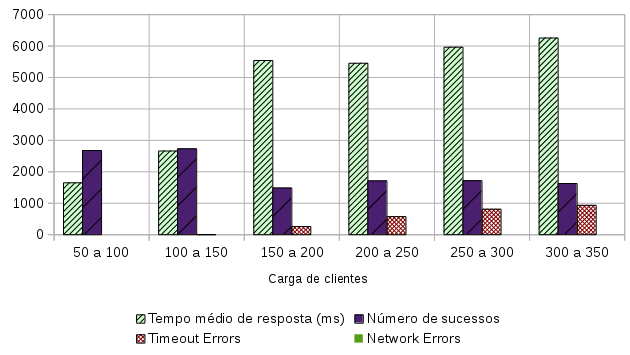
\includegraphics[width=.80\textwidth]{imagem/graficos/grafico_django_plano_de_teste_3.png}
    % Caption centralizada
    \captionsetup[grafico]{justification=centering}
    % Fonte
    \captionfont{\small{\textbf{\\Fonte: Autor}}}
  \end{grafico}
  
  Agora apresentamos o gráfico \ref{grafico:teste-mantendo-carga-usuario-node} referente aos testes realizados com o Node.Js

  \begin{grafico}[H]
    % Alterar espaçamentos antes e depois do caption
    \setlength{\abovecaptionskip}{5pt}
    \setlength{\belowcaptionskip}{0pt}
    \label{grafico:teste-mantendo-carga-usuario-node}
    % Caption
    \caption[Mantendo a carga de usuários no Node.Js]
	    {Mantendo a carga de usuários no Node.Js}
    \centering
    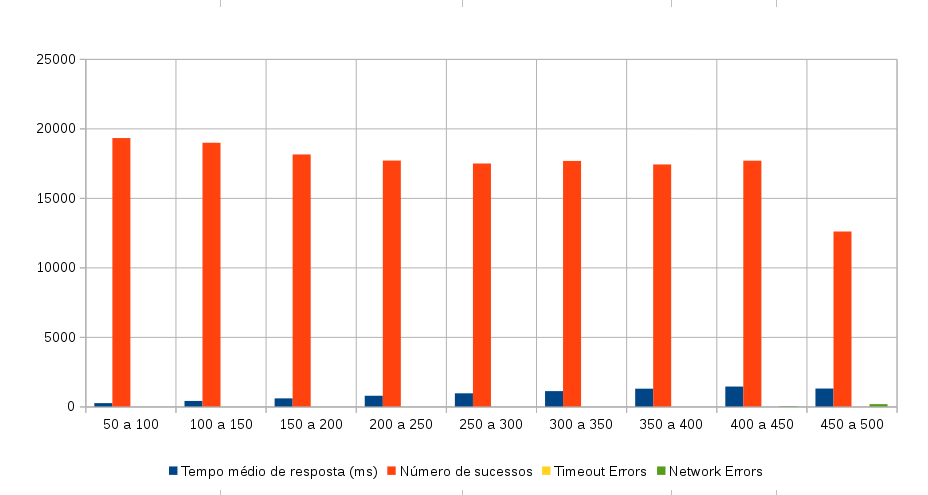
\includegraphics[width=.80\textwidth]{imagem/graficos/grafico_node_plano_de_teste_3.png}
    % Caption centralizada
    \captionsetup[grafico]{justification=centering}
    % Fonte
    \captionfont{\small{\textbf{\\Fonte: Autor}}}
  \end{grafico}
  